%!tex root = ../report.tex

\section{Antipatterns}
\textbf{Developer Antipatterns:}
Focus on the viewpoint of the software developer.\\
Issues: software refactoring, modification of source code to
improve the software structure with respect to long-term
maintainability.\\
\textbf{Architecture Antipatterns}
Focus on the viewpoint of the software architect.\\
Issues: partitioning of subsystems and components, platform
independent definition of interfaces, and connectivity of
components.\\
\textbf{Management Antipatterns}
Focus on the viewpoint of the software project manager.\\
Issues: software project organization, software project
management, software process model, human communication,
rationale management and resolution of issues.\\

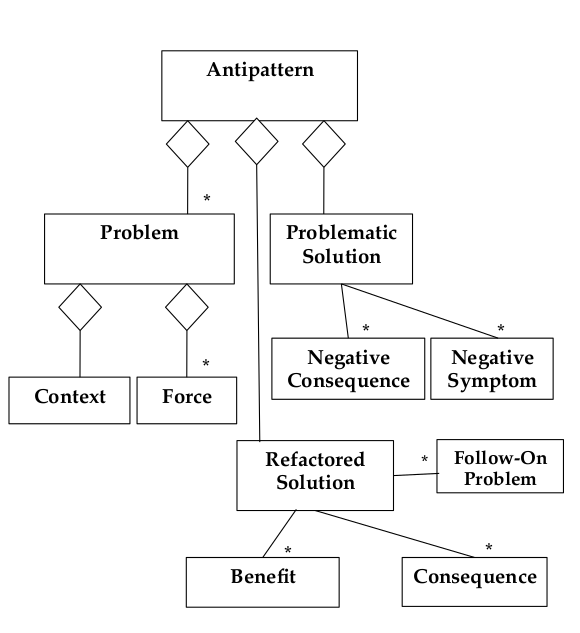
\includegraphics[width=.5\linewidth]{images/antipattern.png}

\textbf{7 Deadly Sins in Software Practice:}
\begin{description}
  \item[Apathy] Not caring about a problem, followed by unwillingness To attempt a solution
  \item[Haste] Solutions based on hasty decisions lead to compromises in software quality
  \item[Narrow-mindedness] The refusal to use solutions that are widely known
  \item[Sloth] Making poor decisions based on "easy" answers
  \item[Avarice (excessive complexity)] no use of abstractions, excessive modeling of details
  \item[Ignorance] Failure to seek understanding
  \item[Pride] Not invented here: not willing to adopt anything from the outside
\end{description}
\newpage

\subsection{Functional Decomposition Antipattern}
Functional decomposition describes the decomposition of a system in terms of functions instead of use cases and/or objects (object-oriented decomposition) so that functions are hidden somewhere in the system where nobody might expect them.\\
recommended approach: first decompose in use cases, then in objects.
\begin{description}
  \item[General Form] Everything is a function, lots of files named misc, util,aux,...
  \item[Symptoms and Consequences] \hfill
  \begin{itemize}
    \item Maintainer must understand the whole system to make changes
     \item Code is hard to understand
     \item Code is complex, high coupling between code sections in different files
     \item User interface is often awkward and non-intuitive
  \end{itemize}
  \item[Typical Causes] Wrong trained personal (programmers, designers)
\end{description}
\newpage

\subsection{Golden Hammer Antipattern}
Everything is solved with a specific tool.
\begin{description}
  \item[General Form] \hfill
  \begin{itemize}
    \item Developer has high level of competence in a particular solution
    \item Every new development effort is solved with this solution
    \item Developer is unwilling to learn and apply new approach
  \end{itemize}
  \item[Symptoms and Consequences] \hfill
  \begin{itemize}
    \item Identical tools used for a many divers products
    \item System architecture depends on a specific tool chain
  \end{itemize}
  \item[Typical Causes] Large investment in product for specific technologies maybe with exclusive features.
  \item[Known Exceptions] Product is part of a vendor suite that provides for all needs
\end{description}
\newpage

\subsection{Lava Flow}
Also known as dead code.
\begin{description}
  \item[General Form] Lava like flows of previous development hardened into a basalt like mass of code, difficult to remove once solidified
  \item[Symptoms and Consequences] \hfill
  \begin{itemize}
    \item Unused or commented-out code
    \item Undocumented complex, important-looking code
    \item Functions or classes that do not relate to the system architecture
    \item evolving architecture
  \end{itemize}
  \item[Typical Causes] \hfill
  \begin{itemize}
    \item Research and development code placed into production
    \item Implementation of several trial approaches
    \item High programmer turnover rate
    \item Fear of breaking something and not knowing how to fix it
    \item Unclear, repeatedly changing project goals
    \item Architectural scars
  \end{itemize}
  \item[Exceptions] Throwaway code
\end{description}
\newpage

\subsection{Blob Antipattern}
Also known as god class
\begin{description}
  \item[General Form] Majority of responsibilities are in one complex controller associated with simple data classes
  \item[Symptoms and Consequences] \hfill
  \begin{itemize}
    \item Huge class with many unrelated attributes and operations encapsulated
    \item The blob is usually to complex to reuse and test
  \end{itemize}
  \item[Typical Causes] \hfill
  \begin{itemize}
    \item Lack of architecture
    \item Too limited intervention in iterative projects
  \end{itemize}
  \item[Known Exceptions] Wrapping of legacy systems
\end{description}
\newpage

\subsection{Spaghetti Code Antipattern}
\begin{description}
  \item[General Form] Software with very little structure where object methods are invoked in a single, multistage process flow
  \item[Symptoms and Consequences] \hfill
  \begin{itemize}
    \item Methods are process oriented, objects are named as processes
    \item Execution flow is dictated by the class implementation of objects instead by the users of that class
    \item No inheritance, no polymorphism
    \item Source code difficult to reuse
    \item Point of diminishing returns: the software maintenance effort is higher than a complete re-engineering effort
  \end{itemize}
  \item[Typical Causes] \hfill
  \begin{itemize}
    \item No design prior to implementation
    \item Inexperience with object-oriented design
  \end{itemize}
\end{description}
\newpage

\subsection{Vendor Lock-In Antipattern}
\begin{description}
  \item[General Form] A software project adopts product technology and becomes completely dependent of the vendor's implementation
  \item[Symptoms and Causes] \hfill
  \begin{itemize}
    \item Maintenance cycle driven by the product update cycle
    \item Promised product features are delayed or never delivered, subsequently, causing failure to deliver application updates
    \item Application programming requires in-depth product knowledge
  \end{itemize}
  \item[Typical Causes] \hfill
  \begin{itemize}
    \item Product is selected because of marketing instead of technical inspection
    \item Product varies from published open system standards because there is no effective conformance process for the standard.
  \end{itemize}
  \item[Known Exceptions] Single vendors code is the majority of the code needed for an application
\end{description}
\newpage

\subsection{Analysis Paralysis Antipattern}
\begin{description}
  \item[General Form] \hfill
  \begin{itemize}
    \item Goal to achieve perfection and completeness of the analysis phase
    \item Very detailed models
  \end{itemize}
  \item[Symptoms and Consequences] \hfill
  \begin{itemize}
    \item Analysis cost exceeds expectations without a predictable end point
    \item Analysis documents no longer make sense to the domain experts
  \end{itemize}
  \item[Typical Causes] \hfill
  \begin{itemize}
    \item Management assumes waterfall progression of phases
    \item Analysis Goals are not well defined
  \end{itemize}
\end{description}
\newpage

\subsection{Code Smells and Refactoring}
\textbf{Code Smells}
\begin{itemize}
  \item Method too long
  \item Duplicated code
  \item Class to large
  \item Parameter list too long
  \item Feature envy (class uses methods of another class excessively)
  \item Lazy class
  \item Speculative generality
  \item Refused bequest (subclass is reusing behavior of the superclass, but does not want to support its interface)
\end{itemize}

\textbf{Refactoring}\\
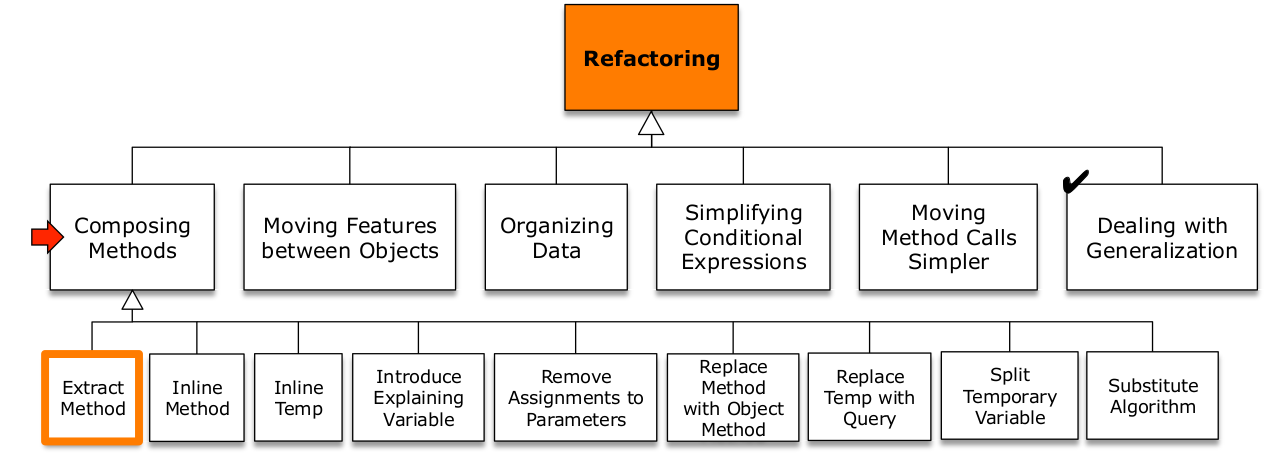
\includegraphics[width=\linewidth]{images/refactoring_composing_methods.png}
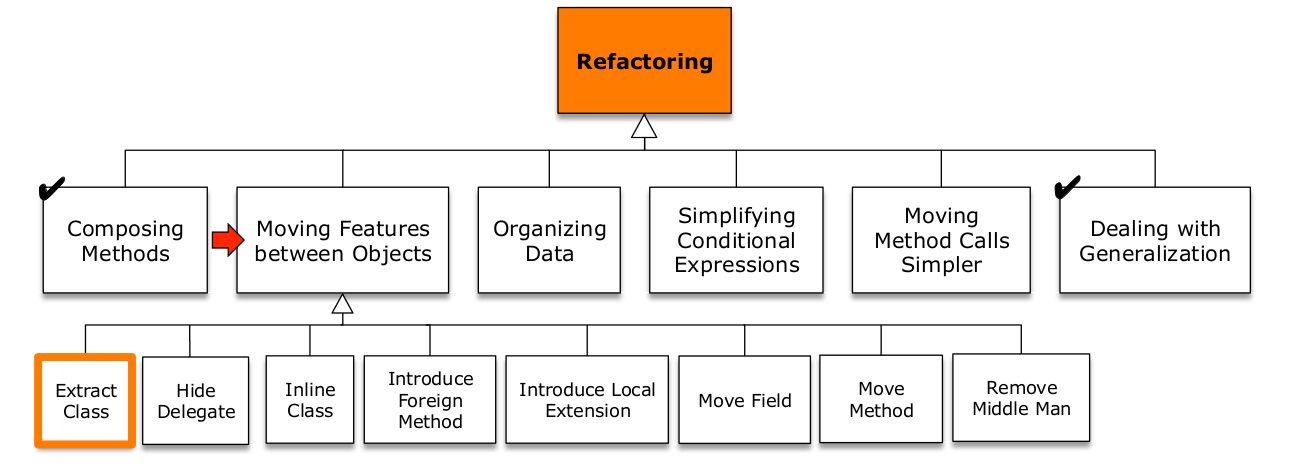
\includegraphics[width=\linewidth]{images/refactoring_moving_features.png}
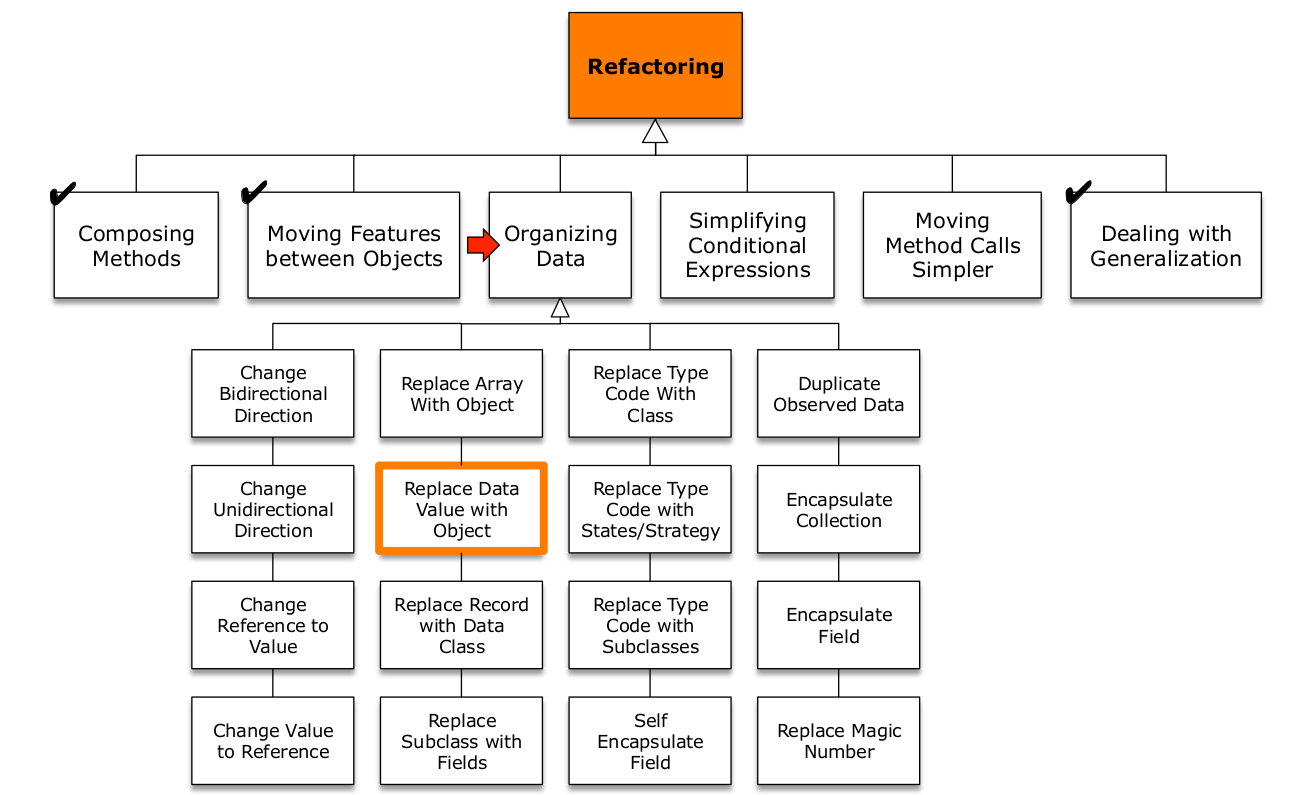
\includegraphics[width=\linewidth]{images/refactoring_organizing_data.png}
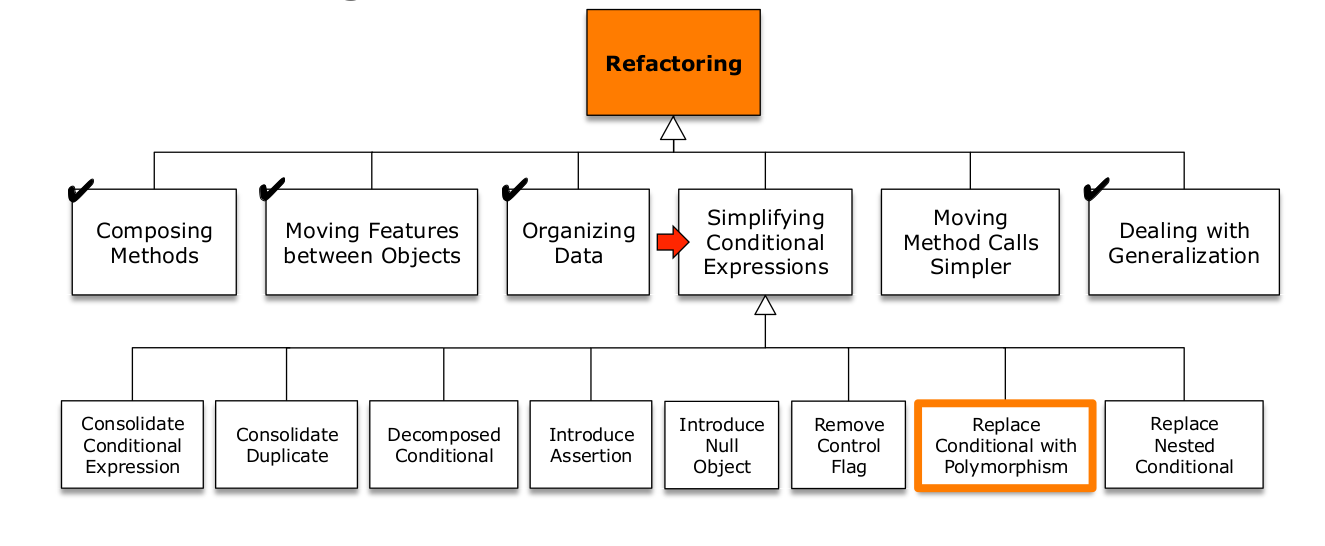
\includegraphics[width=\linewidth]{images/refactoring_conditional_expressions.png}
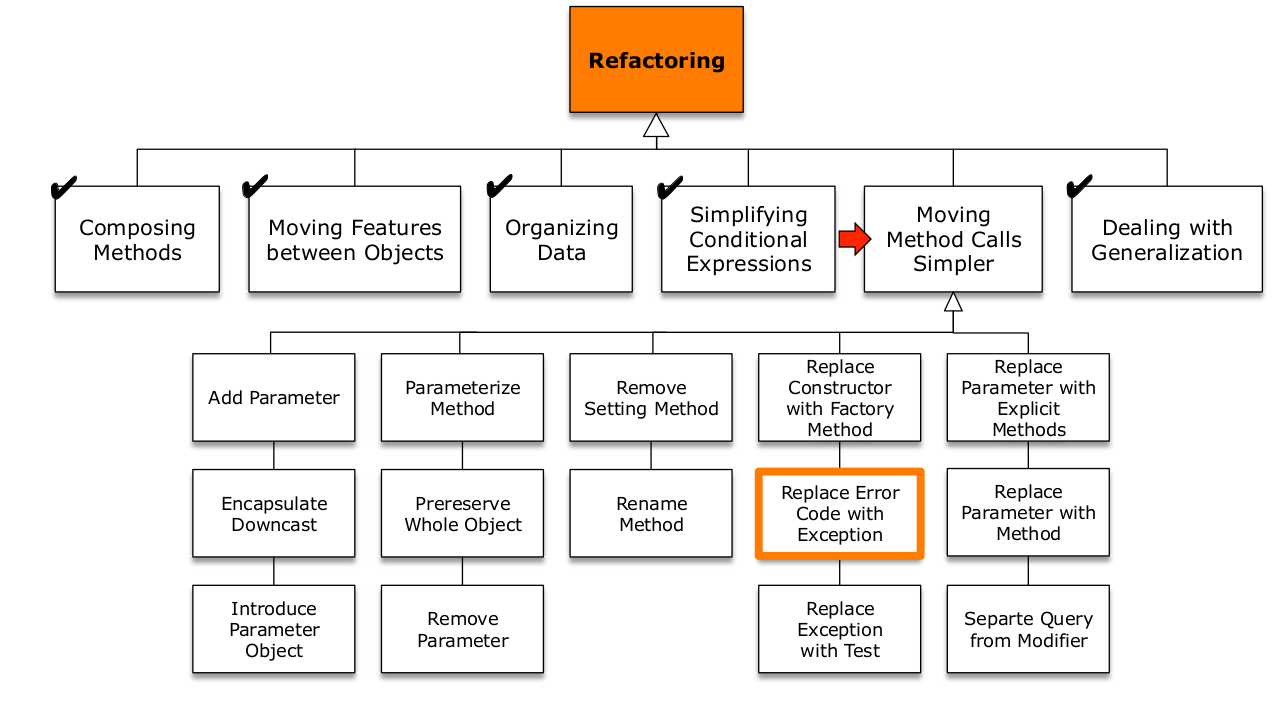
\includegraphics[width=\linewidth]{images/refactoring_moving_method_calls.png}
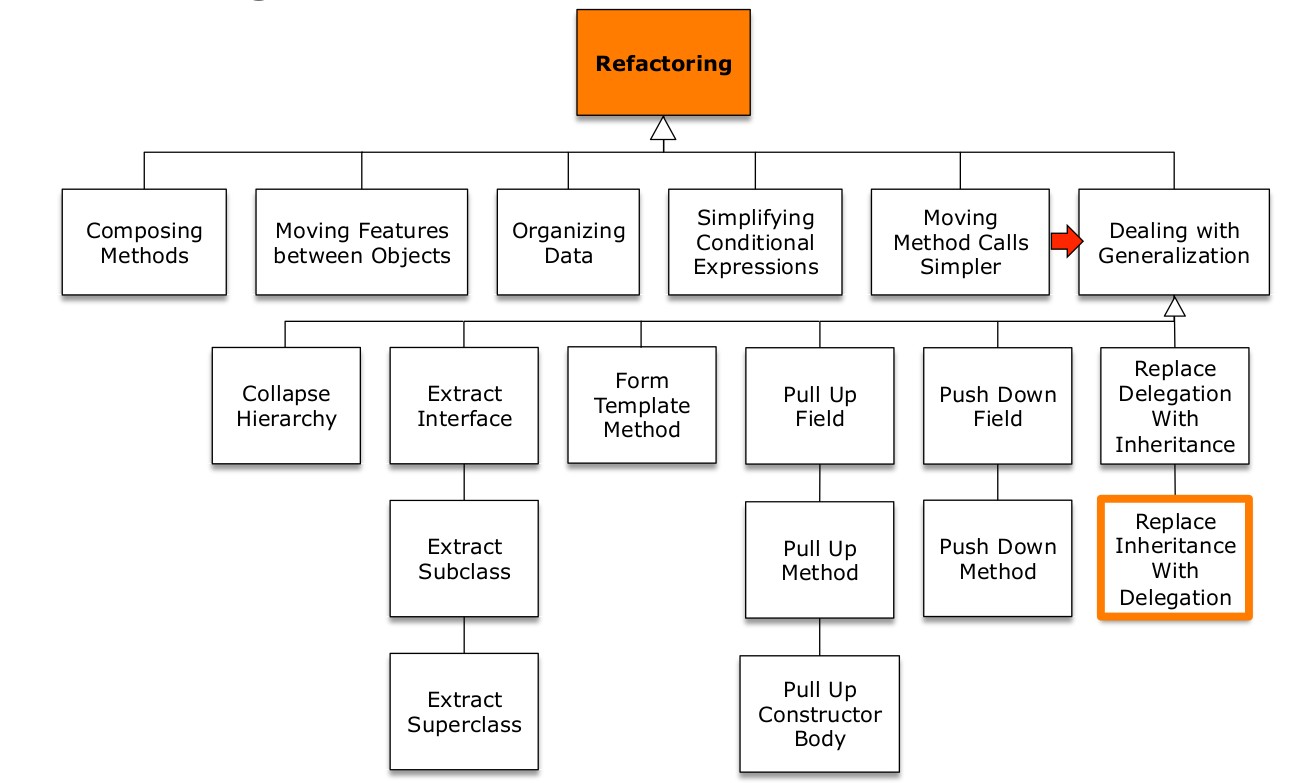
\includegraphics[width=\linewidth]{images/refactoring_generalization.png}
\newpage
